\SubProblem
{د}
{
رابطه آنتروپی مشترک را بررسی می‌کنیم:
    
\begin{equation*}
    H(X) + H(Y|X) = \frac{7}{4} + \frac{13}{8} = \frac{27}{8} [\frac{bits}{symbol}]
\end{equation*}

\begin{equation*}
    H(Y) + H(X|Y) = 2 + \frac{11}{8} = \frac{27}{8} [\frac{bits}{symbol}]
\end{equation*}

\begin{equation}
    H(X, Y) = H(X) + H(Y|X) = H(Y) + H(X|Y)
\end{equation}

    رابطه شماره (1) همان آنتروپی مشترک است.
    این معیار برای بیان میزان ابهام در مورد مجموعه‌ای از متغیرهای تصادفی بکار می‌رود.
    که به صورت شهودی در نمودار ون زیر قابل مشاهده است:

    \begin{figure}[H]
        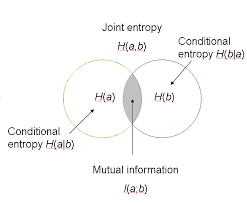
\includegraphics[width=8cm]{Images/Joint_Entropy.png}
        \centering
        \caption{نمودار ون آنتروپی مشترک}
    \end{figure}
}